\chapter{Introducción}
\label{cap:capitulo1}
\setcounter{page}{1}

\begin{flushright}
\begin{minipage}[]{10cm}
\emph{Quizás algún fragmento de libro inspirador...}\\
\end{minipage}\\

Autor, \textit{Título}\\
\end{flushright}

\vspace{1cm}

El ictus es una enfermedad cerebrovascular (ECV).
El término ictus en latín significa golpe.
Es un trastorno brusco de la circulación cerebral que altera la función de una determinada región del cerebro.

Según la Organización Mundial de la Salud (OMS), es la primera causa de discapacidad y la segunda de muerte en el mundo\footnote{\url{https://www.who.int/srilanka/news/detail/29-10-2022-world-stroke-day-2022}}.
Aproximadamente 15 millones de personas sufren un ictus cada año; entre ellas, 5 millones mueren y otros 5 millones quedan con alguna discapacidad permanente, lo que supone una carga significativa para las familias y comunidades\footnote{\url{https://www.emro.who.int/health-topics/stroke-cerebrovascular-accident/index.html}}.

Según el Sistema Nacional de Salud, \cite{perales1a}, cada año, alrededor de $120.000$ personas sufren un ictus en España.
La edad es uno de los factores de riesgo principales de esta enfermedad, aunque ocurre en todos los grupos de edad.
En los últimos años la incidencia en adultos jóvenes ha aumentado un $40\%$.
Los mejores sistemas de diagnóstico, así como el aumento de consumo de drogas, pueden ser algunas de las causas de este aumento.
Se estima que 1 de cada 4 personas en el mundo sufrirán un ictus a lo largo de su vida.
Gracias a los avances científicos, tecnológicos y clínicos se han podido desarrollar tratamientos para minimizar los déficits que produce.
En la Imagen \ref{fig:grafica}, se muestra la prevalencia registrada de enfermedad cerebrovascular por 1.000 habitantes, según sexo y edad en España en 2019.

\begin{figure}[ht!]
	\centering
	\begin{minipage}{0.95\linewidth}
		\centering
		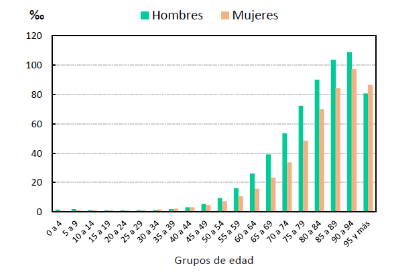
\includegraphics[width=\linewidth]{figs/edad_ictus_es.png}
	\end{minipage}
	\caption{Prevalencia registrada de enfermedad cerebrovascular según sexo y edad en España, 2019}
	\label{fig:grafica}
\end{figure}

Según el Grupo de Estudio de ECV de la Sociedad Española de Neurología (SEN), para la mayoría de los pacientes que han sufrido un ictus y han sobrevivido, la rehabilitación es una de las partes más importantes de su tratamiento.
Suele comenzarse en los primeros días de estancia en el hospital y se recomienda a cualquier paciente que, previo al ictus, fuese autosuficiente.
Es importante entender que es difícil volver a una situación igual a la inicial.
El objetivo fundamental es ayudar al paciente a adaptarse, ya que el ictus se recupera de forma espontánea o puede no recuperarse nunca, dependiendo de su gravedad, la cual determina la duración del programa de rehabilitación y su intensidad.
Los seis primeros meses son los de mayor importancia para recuperar los movimientos voluntarios.
Con un programa adecuado, un $1/3$ de los pacientes vuelven a su trabajo.

El plan de acción europeo para el ictus 2018-2030, propuesto por la Alianza Europea contra el ictus \cite{perales1b}, surge con el objtivo de mejorar el cuidado de los ictus y la vida después de estos.
Entre los objetivos generales para el año 2030 se encuentran:
\begin{enumerate}
    \item Garantizar que al menos el $90\%$ de la población tenga acceso a la rehabilitación precoz en la unidad de ictus.
    \item Proporcionar el alta precoz con apoyo a por lo menos el $20\%$ de los pacientes de ictus en todos los países.
    \item Ofrecer programas de acondicionamiento físico a todos los pacientes de ictus que viven en la comunidad.
    \item Proporcionar un plan documentado para la rehabilitación en la comunidad y el apoyo al autocontrol de todos los pacientes de ictus con dificultades residuales al recibir el alta hospitalaria.
    \item Garanticen que se revisan las necesidades de rehabilitación, y otras, de todos los pacientes de ictus entre los 3 y 6 meses después de sufrirlo y anualmente a partir de ese momento.
\end{enumerate}\

Una de las consecuencias de sufrir un ictus son los trastornos motores.
La debilidad o pérdida de fuerza en una extremidad o la cara son síntomas frecuentes en estos pacientes.
Al principio, tienen poco tono muscular y más aelante se produce una contracción progresiva de los músculos y se acentúa con movimientos bruscos.
Esto último debe tenerse en cuenta a la hora de modelar una sesión de rehabilitación.\footnote{\url{http://ictus.sen.es}}

[Hablar de la inclusión de sistemas robóticos como herramienta terapéutica, mejoras en las sesiones, concretar sobre entornos de gamificación.]
